% \documentclass[conference]{IEEEtran}
\documentclass[12pt]{article}
\usepackage[utf8]{inputenc}
\usepackage{graphicx}
\graphicspath{ {images/} }

% The preceding line is only needed to identify funding in the first footnote. If that is unneeded, please comment it out.
% \usepackage{cite}
\usepackage{amsmath,amssymb,amsfonts}
\usepackage{algorithmic}
\usepackage{graphicx}
\usepackage{textcomp}
\usepackage{xcolor}

% user self defined
\usepackage{hyperref}
% \hypersetup{hidelinks=true}
\usepackage{booktabs}
\usepackage{tabularx}
\usepackage{caption}
\usepackage{subcaption}

% \usepackage{biblatex}
%Citation-related commands
\usepackage[style=ieee]{biblatex}
\addbibresource{ref.bib}
% \def\BibTeX{{\rm B\kern-.05em{\sc i\kern-.025em b}\kern-.08em
%     T\kern-.1667em\lower.7ex\hbox{E}\kern-.125emX}}
\begin{document}

\title{
{Bachelor Thesis Draft}\\
{\large Maastricht University}\\
% {
\includegraphics{UMlogo.jpg}}
}
\author{Yiping Huang}
% \IEEEauthorblockA{\textit{Department of Data Science and Artificial Intelligence} \\
% \textit{Maastricht University}\\
% Maastricht, The Netherlands}
% }

\maketitle

% \chapter*{Abstract}

% \chapter*{Dedication}
% To mum and dad

% \chapter*{Declaration}
% I declare that..

% \chapter*{Acknowledgements}
% I want to thank...

\tableofcontents

% \begin{abstract}
% The document reports the test results of the EA(Evolutionary Algorithm) on different instances of problems, i.e., the 0-1 knapsack problems and the TSP(Traveling Salesman Problem).
% \end{abstract}

% \begin{IEEEkeywords}
% EA, 0-1 knapsack problem, TSP problem, Combinatorial Optimization
% \end{IEEEkeywords}


% \begin{table}[h!]
%     \centering
%     \begin{tabular}{lrrr}
  \toprule
                    file &  ga\_sol &  actual\_sol &  deviation \\
  \midrule
    knapPI\_1\_5000\_1000\_1 &  221927 &      276457 &                  0.20 \\
     knapPI\_2\_100\_1000\_1 &    1512 &        1514 &                  0.00 \\
    knapPI\_2\_2000\_1000\_1 &   17022 &       18051 &                  0.06 \\
     knapPI\_3\_200\_1000\_1 &    2693 &        2697 &                  0.00 \\
     knapPI\_1\_500\_1000\_1 &   27553 &       28857 &                  0.05 \\
     knapPI\_1\_200\_1000\_1 &   11238 &       11238 &                  0.00 \\
   knapPI\_1\_10000\_1000\_1 &  440860 &      563647 &                  0.22 \\
    knapPI\_1\_2000\_1000\_1 &   94002 &      110625 &                  0.15 \\
    knapPI\_3\_1000\_1000\_1 &   13376 &       14390 &                  0.07 \\
    knapPI\_2\_5000\_1000\_1 &   41280 &       44356 &                  0.07 \\
     knapPI\_3\_500\_1000\_1 &    6914 &        7117 &                  0.03 \\
   knapPI\_2\_10000\_1000\_1 &   81867 &       90204 &                  0.09 \\
    knapPI\_3\_2000\_1000\_1 &   26016 &       28919 &                  0.10 \\
     knapPI\_3\_100\_1000\_1 &    2390 &        2397 &                  0.00 \\
    knapPI\_1\_1000\_1000\_1 &   49987 &       54503 &                  0.08 \\
   knapPI\_3\_10000\_1000\_1 &  124091 &      146919 &                  0.16 \\
     knapPI\_2\_200\_1000\_1 &    1634 &        1634 &                  0.00 \\
    knapPI\_3\_5000\_1000\_1 &   62798 &       72505 &                  0.13 \\
    knapPI\_2\_1000\_1000\_1 &    8761 &        9052 &                  0.03 \\
     knapPI\_2\_500\_1000\_1 &    4495 &        4566 &                  0.02 \\
     knapPI\_1\_100\_1000\_1 &    8929 &        9147 &                  0.02 \\
  \bottomrule
  \end{tabular}
      
%     \caption{Deviation with population size =$ 10$}        
%     \label{table:pop10_deviation}
%     \end{table}
% \begin{table}[h!]
%     \centering
%     \begin{tabular}{lrrrr}
  \toprule
                    file &  found &  ga\_weight &  actual\_weight &  time \\
  \midrule
    knapPI\_1\_5000\_1000\_1 &     76 &      24849 &          25016 &  9.05 \\
     knapPI\_2\_100\_1000\_1 &     24 &        953 &            991 &  0.27 \\
    knapPI\_2\_2000\_1000\_1 &     78 &      10009 &          10010 &  4.42 \\
     knapPI\_3\_200\_1000\_1 &     84 &        993 &            997 &  0.45 \\
     knapPI\_1\_500\_1000\_1 &     85 &       2498 &           2543 &  1.11 \\
     knapPI\_1\_200\_1000\_1 &      4 &        987 &            987 &  0.48 \\
   knapPI\_1\_10000\_1000\_1 &     63 &      49714 &          49877 & 19.99 \\
    knapPI\_1\_2000\_1000\_1 &     87 &      10003 &          10011 &  3.93 \\
    knapPI\_3\_1000\_1000\_1 &     43 &       4976 &           4990 &  2.04 \\
    knapPI\_2\_5000\_1000\_1 &     99 &      24999 &          25016 & 10.28 \\
     knapPI\_3\_500\_1000\_1 &     74 &       2514 &           2517 &  1.14 \\
   knapPI\_2\_10000\_1000\_1 &     76 &      49703 &          49877 & 19.91 \\
    knapPI\_3\_2000\_1000\_1 &     73 &       9816 &           9819 &  3.90 \\
     knapPI\_3\_100\_1000\_1 &     22 &        990 &            997 &  0.24 \\
    knapPI\_1\_1000\_1000\_1 &     78 &       4965 &           5002 &  1.98 \\
   knapPI\_3\_10000\_1000\_1 &     44 &      49491 &          49519 & 19.76 \\
     knapPI\_2\_200\_1000\_1 &     67 &       1006 &           1006 &  0.45 \\
    knapPI\_3\_5000\_1000\_1 &     64 &      24798 &          24805 &  9.71 \\
    knapPI\_2\_1000\_1000\_1 &     98 &       4993 &           5002 &  2.17 \\
     knapPI\_2\_500\_1000\_1 &     55 &       2539 &           2543 &  1.03 \\
     knapPI\_1\_100\_1000\_1 &      3 &        972 &            985 &  0.24 \\
  \bottomrule
  \end{tabular}
%     \caption{running time(s) for $100$ generations with population size $10$}
%     \label{table:pop10_time}
% \end{table}

% \begin{figure}[h]
%     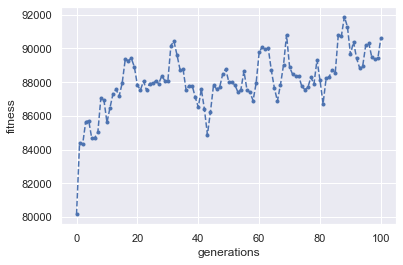
\includegraphics[width=8cm]{image/average_fitness_pop10.png}
%     \caption{Average Fitness Change (population size = $10$) with File knapPI\_1\_2000\_1000\_1 as Input}
%     \label{image:fitness_pop10}
%     \end{figure}


% \begin{figure}[h]
%     \centering
%     \begin{subfigure}[b]{0.3\textwidth}
%         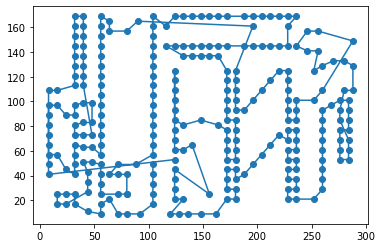
\includegraphics[width=\textwidth]{image/tsp/ga_result.png}
%         \caption{Best Solution Found}
%         \label{image:best solution}
%     \end{subfigure}
    
%     \begin{subfigure}[b]{0.3\textwidth}
%         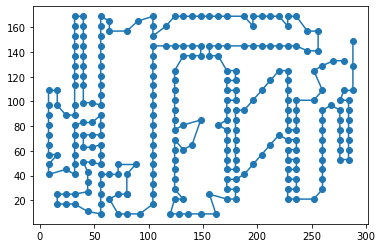
\includegraphics[width=\textwidth]{image/tsp/optimal_solution.png}
%         \caption{Optimal Solution}
%         \label{image:optimal solution}
%         \end{subfigure}        
% \end{figure}
% \chapter{Literature Review}
\section{Literature Review}
\subsection{Modularity}
Communities are often considered as tightly connected components within the whole structure. 

Modularity Q measures how well the network is partitioned into communities. It is based on the assumption that community members tend to connect more with each other than with members from outside the community, which is often true in our daily life. Thus it can be expressed as  
\[ Q \propto \sum_{s\in S}^{} (\text{\#edges within s}) - E(\text{\#edges within s})\], where $S$ is the partition set. a model that is based on this criteria gives us a high $Q$ value.

To define the expection of edges between two nodes, we need to pick up a null model. One way is to connect nodes in a completely random way but each node needs to maintain its original degree\cite{newman2006modularity}. So in this null model, multiple edges between nodes are allowed to exist, which turns the original graph into a multi-graph. For a graph with $n$ nodes and $m$ edges, the expected edges between Node $i$ and $j$ would be $\frac{k_ik_j}{2m}$, where $k_i$ is the degree for node $i$. This is because the probability for one stub of node $i$ hitting the target node $j$ is $\frac{K_j}{2m}$, and summing over all stubs of node $i$ we have $k_i\cdot\frac{k_j}{2m}$. Then given a partition $S$, $Q(G,S)$ is defined as 
\begin{equation} \label{basic}
    Q = \frac{1}{2m}\sum_{s\in S} \sum_{i\in s}\sum_{j \in s} (A_{ij} - \frac{k_ik_j}{2m})    
\end{equation}
     where $A_{ij}$ is $1$ if node $i$ is pointing towards node $j$ and $0$ otherwise. Equivalently, this can be written as 
\begin{equation}
    Q = \sum_{s \in S}\frac{\sum_{in}}{2m} - {(\frac{\sum_{tot}}{2m})}^2   
\end{equation}, where $\sum_{in}$ denotes sum of link weights between nodes in the set $s$, and $\sum_{tot}$ denotes sum of all link weights of nodes in the set $s$. This is because 
$\sum_{i \in s}\sum_{j \in s}A_{ij} = \sum_{in}$ 
and 
\begin{equation*}
    \begin{split}
     & \sum_{i \in s}\sum_{j \in s} k_ik_j \\
     = & \sum_{i \in s} k_i \sum_{j \in s} k_j \\
     = & {\sum_{tot}}^2
    \end{split}
\end{equation*}

% \[Q = \frac{1}{2m}\sum_{ij}[A_{ij} - \frac{k_ik_j}{2m}]\delta(c_i, c_j) \]
% where $c_i$ is the community of node $i$ and $\delta(c_i, c_j)$ is $1$ if $c_i = c_j$.
\subsection{Louvain Algorithm}
Louvain algorithm \cite{blondel2008fast} is a fast optimization technique to maximize the modularity. It consists of two phases, namely, one partitioning phase and one restructuring phase. The first phase iterates through all the nodes, and for each node, tries to find the community that results in the maximum modularity gain. It then moves that node into that community and proceeds the next node. This process iterates until no node is found to move to another community. Then the second phase kicks in. This phase simply groups all nodes found in the community into a supernode, and turns edges within the community into self-loop edge for the supernode, and connect two supernodes only when there exists a pair of nodes between the two communities that connect to each other. The new edge weight is the sum of all the corresponding edge weights within or between the communities. This two-step process then repeats until the whole graph morphes to a single supernode. 

The louvain algorithm is a greedy algorithm in that at each step it only moves the node to the community that maximize the modularity gain. It is fast since the modularity gain can be calculated quite easily once we calculated the total degrees and in degrees.

The modularity gain from moving an isolated node $i$ to a new community $c$ is then
\begin{equation} \label{movein}
    [\frac{\sum in+k_{i,in} }{2m} - {(\frac{\sum_{tot} + k_i}{2m})}^2] - [\frac{\sum_{in}}{2m} - (\frac{\sum_{tot}}{2m})^2 - {(\frac{k_i}{2m})}^2]
\end{equation}, similarly the modularity gain from from moving a node $i$ out of a community $d$ is then
\begin{equation} \label{moveout}
    [\frac{\sum_{in} - k_{i,in}}{2m} - {(\frac{\sum_{tot}-k_i}{2m})}^2 - {(\frac{k_i}{2m})}^2] - [\frac{\sum_{in}}{2m} - {(\frac{\sum_{tot}}{2m})}^2]
\end{equation}
The modularity gain from moving a node $i$ from its community $d$ to community $c$ is then the sum of \ref{movein} and \ref{moveout}. As we can see, we only need to store the $\sum_{in}$ and $\sum_{tot}$ for all the communities in the beginning of phase one, and the change in modularity is then easy to compute without invoking \ref{basic} to compute the modularity from scratch each time we try out different possibility.




\appendix
% \chapter{Appendix Title}
% \input{sections/appendix}

% \bibliographystyle{IEEEtran}
% \bibliography{ref}
\printbibliography
\end{document}
